%%%%%%%%%%%%%%%%%%%%%%%%%%%%%%%%%%%%%%%%%%%%%%%%%%%%%%%%%%%%%%%%%%%%%%%%%%%%%%%%
%% Title (en): Multiagent Systems and Organizations                           %%
%% Title (cs): Multiagentní systémy a organizace                              %%
%%                                                                            %%
%% Author: Bc. Lukáš Kúdela                                                   %%
%% Supervisor: Prof. RNDr. Petr Štěpánek, DrSc.                               %%
%%                                                                            %%
%% Academic year: 2011/2012                                                   %%
%%%%%%%%%%%%%%%%%%%%%%%%%%%%%%%%%%%%%%%%%%%%%%%%%%%%%%%%%%%%%%%%%%%%%%%%%%%%%%%%

%%%%%%%%%%%%%%%%%%%%%%%%%%%%%%%%%%%%%%%%%%%%%%%%%%%%%%%%%%%%%%%%%%%%%%%%%%%%%%%%
\section{Example 3: Auction}
%%%%%%%%%%%%%%%%%%%%%%%%%%%%%%%%%%%%%%%%%%%%%%%%%%%%%%%%%%%%%%%%%%%%%%%%%%%%%%%%

% Auction organization
This example demonstrates a relatively complex organization - the auction.
% Auction organization - purpose
The purpose of this organization is to facilitate auction by bringing together several agents: one agent auctions an item and the other agents bid for it.
The item can be auctioned in an envelope, Vickrey, english or dutch auction.
% Assumptions
In this example, agents sell and buy works of art (famous paintings) in an envelope auction, but it should be obvious that any of the four auction types could be used to sell any items.

%%%%%%%%%%%%%%%%%%%%%%%%%%%%%%%%%%%%%%%%%%%%%%%%%%%%%%%%%%%%%%%%%%%%%%%%%%%%%%%%
\subsection*{Specification}

%%%%%%%%%%%%%%%%%%%%%%%%%%%%%%%%%%%%%%%%%%%%%%%%%%%%%%%%%%%%%%%%%%%%%%%%%%%%%%%%
\subsubsection*{Organization Part}

% 'Auction' organizaiton type
The \textit{Auciton} organization type (modelled by the \texttt{Auction\_Organization} agent class) contains two roles - \textit{Auctioneer} and \textit{Bider} - and four protocols - \textit{Envelope auction}, \textit{Vickrey auction}, \textit{English auction} and \textit{Dutch auction}.
% 'auction' organization
\textit{Auction} has one instance in the running MAS - the \textit{auction} organization (modelled by the \texttt{auction\_Organization} agent instance).

% 'Auctioneer' role
The \textit{Auctioneer} role (modelled by the \texttt{Auctioneer\_Role} class) can sell an item in an auction, i.e. it can auction an item.
% 'Auctioneer' role - multiplicity, competences & responsibilities
The \textit{Auctioneer} role is a \textit{single} role.
It has one competence - \textit{Auction} - and no responsibilities.

% 'Auction' competence
The \textit{Auction} competence (modelled by the \texttt{Auction\_Competence} class) is a competence to auction an item.
% 'Auction' competence - argument & result
It has several arguments depending on the type of the auction - mainly the name of the item - and several results - particularly the hammer price.

% 'Bidder' role
The \textit{Bidder} role (modelled by the \texttt{Bidder\_Role} class) can buy an item in an auction, i.e. it can bid for an item. 
% 'Bidder' role - multiplicity, competences & responsibilities
The \textit{Bidder} role is a \textit{multiple} role.
It has no competences and one responsibility - \textit{Bid}.

% 'Bid' responsibility
The \textit{Bid} responsibility (modelled by the \texttt{Bid\_Responsibility} class) is a responsibility to bid for an item.
% 'Bid' responsibility - argument & result
It has several arguments depending on the type of the auction - mainly the name of the item - and several results - the bid in particular.

%%%%%%%%%%%%%%%%%%%%%%%%%%%%%%%%%%%%%%%%%%%%%%%%%%%%%%%%%%%%%%%%%%%%%%%%%%%%%%%%
\subsubsection*{Protocol Part}

% 'Envelope acution' protocol
The \textit{Envelope auction} protocol (modelled by the \texttt{EnvelopeAuctionProtocol} class) is a protocol through which an \textit{Auctioneer} (the initiator party, modelled by the \texttt{EnvelopeAuction_InitiatorParty} class) can determine the best buyer from among the \textit{Bidders} (responder party, modelled by the \texttt{EnvelopeAuction_RespoderParty} class).
% Envelope auction
The Envelope auction is a sealed bid first-price auction.
In this type of auction the sealed bids (unknown to other bidders) are submitted simultaneously to the auctioneer and the item is sold to the winning bidder for the price of their bid.

% Vickrey auction protocol
The \textit{Vickrey auction} protocol (modelled by the \texttt{VickreyAuctionProtocol} class) is a protocol through which an \textit{Auctioneer} (the initiator party, modelled by the \texttt{VickreyAuction_InitiatorParty} class) can choose the best buyer from among the \textit{Bidders} (responder party, modelled by the \texttt{VickreyAuction_RespoderParty} class).
% Vickrey auction
The Vickrey auction is a sealed bid second-price auction.
In this type of auction the sealed bids are submitted simultaneously to the auctioneer and the item is sold to the winning bidder for the price of the \textit{second} highest bid.

% English auction protocol
The \textit{English auction} protocol (modelled by the \texttt{EnglishAuctionProtocol} class) is a protocol through which an \textit{Auctioneer} (the initiator party, modelled by the \texttt{EnglishAuction_InitiatorParty} class) can determine the best buyer from among the \textit{Bidders} (responder party, modelled by the \texttt{EnglishAuction_RespoderParty} class).
% English auction
The English auction is an open bid ascending price auction.
In this type of auction the auctioneer announces the starting price (lower than the expected selling price).
The bidders then sequentially submit open bids in ascending fashion, respecting the minimum increment.
The item is sold to the \textit{last} bidder willing to pay the price.

% Dutch auction protocol
The \textit{Dutch auction} protocol (modelled by the \texttt{DutchAuctionProtocol} class) is a protocol through which an \textit{Auctioneer} (the initiator party, modelled by the \texttt{DutchAuction_InitiatorParty} class) can determine the best buyer from among the \textit{Bidders} (responder party, modelled by the \texttt{DutchAuction_RespoderParty} class).
% Dutch auction
The Dutch auction is an open bid descending price auction.
In this type of auction the auctioneer announces a starting price (higher than the expected selling price).
The auctioneer then sequentially offers prices in descending fashion, respecting the minimum decrement.
The item is sold to the \textit{first} bidder willing to pay the price.

% 'Auction call-for-proposals' message
The \textit{Auction call-for-proposals (CFP)} message (modelled by the \texttt{AuctionCFPMessage} class) is a message sent by an \textit{Auctioneer} to all \textit{Bidders} calling for proposals for the auctioned item's price.

% 'Bid propose' message
The \textit{Bid propose} message (modelled by the \texttt{BidProposeMessage} class) is a message sent by a \textit{Bidder} to an \textit{Auctioneer} proposing a bid to the latter.

%%%%%%%%%%%%%%%%%%%%%%%%%%%%%%%%%%%%%%%%%%%%%%%%%%%%%%%%%%%%%%%%%%%%%%%%%%%%%%%%
\subsubsection*{Player Part}

% 'Participant' player type
The \textit{Participant} player type (modelled by the \texttt{Participant} agent class) is a player capable of biding for an item.
\textit{Participant} has three instances in the running MAS - \textit{player1}, \textit{player2} and \textit{player3}.
All of them intend to enact both the \textit{Auctioneer} and \textit{Bidder} roles in the \textit{auction} organization and perform the \textit{Auctioneer} role's \textit{Auction} competence - to auction an item to the players of the \textbf{Bidder} role.
They also intend to perform the \textit{Bidder} role's \textit{Bid} responsibility - to bid for an item auctioned by the player of the \textit{Auctioneer} role.
% 'player1' player
\textit{player1} (modelled by the \texttt{player1} agent instance) intends to play the \textbf{Auctioneer} in the first round and be the \textbf{Bidder} in the second and third rounds.
% 'player2' player
\textit{player2} (modelled by the \texttt{player2} agent instance) intends to be the \textit{Auctioneer} in the second round and play the \textit{Bidder} in the first and third rounds.
% 'player3' player
\textit{player3} (modelled by the \texttt{player3} agent instance) intends to play the \textit{Auctioneer} in the third rounds and be the \textit{Bidder} in the first and second rounds.

%%%%%%%%%%%%%%%%%%%%%%%%%%%%%%%%%%%%%%%%%%%%%%%%%%%%%%%%%%%%%%%%%%%%%%%%%%%%%%%%
\section{Manifestation} 

%%%%%%%%%%%%%%%%%%%%%%%%%%%%%%%%%%%%%%%%%%%%%%%%%%%%%%%%%%%%%%%%%%%%%%%%%%%%%%%%
\subsubsection*{Stage 3: Competence and Responsibility Invocation}

% Figure: Stage 3: Competence and responsibility invocation
\begin{figure}[H]
	\centering
	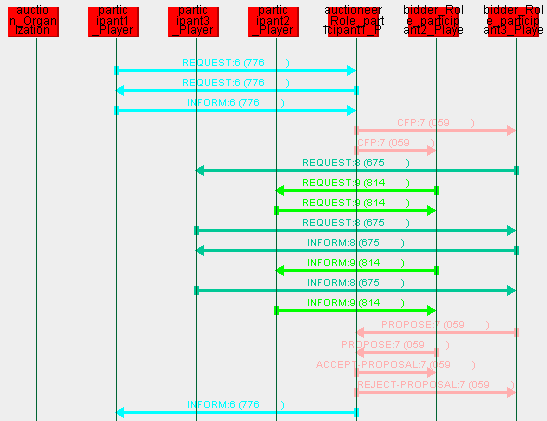
\includegraphics[width=\textwidth]{images/example3-stage3.png}
	\caption{Stage 3: Competence and responsibility invocation}
	\label{figure:example3-stage3}
\end{figure}

% Cyan
\textbf{Cyan} The cyan interaction scenario between the \textit{participant1} player and the \textit{auctioneer-participant1} position follows the \textit{Invoke competence} protocol.
\textit{participant1} requests \textit{auctioneer-participant1} to invoke the \textit{Auction} competence and informs the position about the competence argument - the name of the work of art and the reserve price.
After \textit{auctioneer-participant1} executes the competence (the pink interaction scenario), it informs \textit{participant1} about the competence result - the AID of the winning bidder and the selling price.

% Pink
\textbf{Pink} The pink interaction scenario among the \textit{auctioneer-participant1}, \textit{bidder-participant2} and \textit{bidder-participant3} positions.
\textit{auctioneer-participant1} calls for proposals from \textit{bidder-participant2} and \textit{bidder-participant3} (1\textsuperscript{st} and 2\textsuperscript{nd} messages).
Both \textit{bidder-participant2} and \textit{bidder-participant} then invoke the \textbf{Bid} responsibility on their respective players (the green and teal interaction scenarios respectively) and propose their bids to \textit{auctioneer-participant3} (3\textsuperscript{rd} and 4\textsuperscript{th} messages).
\textit{auctioneer-participant1} then determines the winning bidder, accepts their proposal (5\textsuperscript{th} message) and rejects the other bidders' proposals (6\textsuperscript{th} message).

% Green
\textbf{Green} The green interaction scenario between the \textit{bidder-participant2} position and the \textit{participant2} player follows the \textit{Invoke responsibility} protocol.
\textit{bidder-participant2} requests \textit{participant2} to invoke the \textit{Bid} responsibility and informs the player about the responsibility argument - the name of the work of art.
After \textit{participant2} execute the responsibility, it informs \textit{bidder-participant2} about the responsibility result - the bid.

% Teal
\textbf{Teal} The teal interaction scenario between the \textit{bidder-participant3} position and the \textit{participant3} player follows the \textit{Invoke responsibility} protocol.
This interaction scenario is similar to the green interaction scenario.

% Invoke competence protocol & Invoke responsibility protocol - details
For details about the \textit{Invoke competence} and \textit{Invoke responsibility} protocol see Stage 3 of the first example.